\subsection{Experimental Setup}
\label{sec:setup}

We use a server that has two $16$-core x86-based Intel Xeon Gold 6226R processors running at $2.90$ GHz. Each core has an L1 cache of $1$ MB, an L2 cache of $16$ MB, and a shared L3 cache of $22$ MB. The machine has $93.4$ GB of system memory and runs on CentOS Stream 8. We use GCC 8.5 and OpenMP 4.5. Table \ref{tab:dataset} shows the graphs we use in our experiments. All of them are obtained from the SuiteSparse Matrix Collection \cite{kolodziej2019suitesparse}.

\begin{table}[!ht]
  \centering
  \caption{In our experiments, we use a list of 17 graphs. Each graph has its edges duplicated in the reverse direction to make them undirected, and a weight of 1 is assigned to each edge. The table lists the total number of vertices ($|V|$), total number of edges ($|E|$) after making the graph undirected, and the file size ($F_{size}$) for each graph. The number of vertices and edges are rounded to the nearest thousand or million, as appropriate.}
  \label{tab:dataset}
  \begin{tabular}{|c||c|c|c|}
    \toprule
    \textbf{Graph} &
    \textbf{\textbf{$|V|$}} &
    \textbf{\textbf{$|E|$}} &
    \textbf{\textbf{$F_{size}$}} \\
    \midrule
    \multicolumn{4}{|c|}{\textbf{Web Graphs (LAW)}} \\ \hline
    indochina-2004$^*$ & 7.41M & 341M & 2.9 GB \\ \hline
    arabic-2005$^*$ & 22.7M & 1.21B & 11 GB \\ \hline
    uk-2005$^*$ & 39.5M & 1.73B & 16 GB \\ \hline
    webbase-2001$^*$ & 118M & 1.89B & 18 GB \\ \hline
    it-2004$^*$ & 41.3M & 2.19B & 19 GB \\ \hline
    sk-2005$^*$ & 50.6M & 3.80B & 33 GB \\ \hline
    \multicolumn{4}{|c|}{\textbf{Social Networks (SNAP)}} \\ \hline
    com-LiveJournal & 4.00M & 69.4M & 480 MB \\ \hline
    com-Orkut & 3.07M & 234M & 1.7 GB \\ \hline
    \multicolumn{4}{|c|}{\textbf{Road Networks (DIMACS10)}} \\ \hline
    asia\_osm & 12.0M & 25.4M & 200 MB \\ \hline
    europe\_osm & 50.9M & 108M & 910 MB \\ \hline
    \multicolumn{4}{|c|}{\textbf{Protein k-mer Graphs (GenBank)}} \\ \hline
    kmer\_A2a & 171M & 361M & 3.2 GB \\ \hline
    kmer\_V1r & 214M & 465M & 4.2 GB \\ \hline
  \bottomrule
  \end{tabular}
  \end{table}


\begin{figure*}[hbtp]
  \centering
  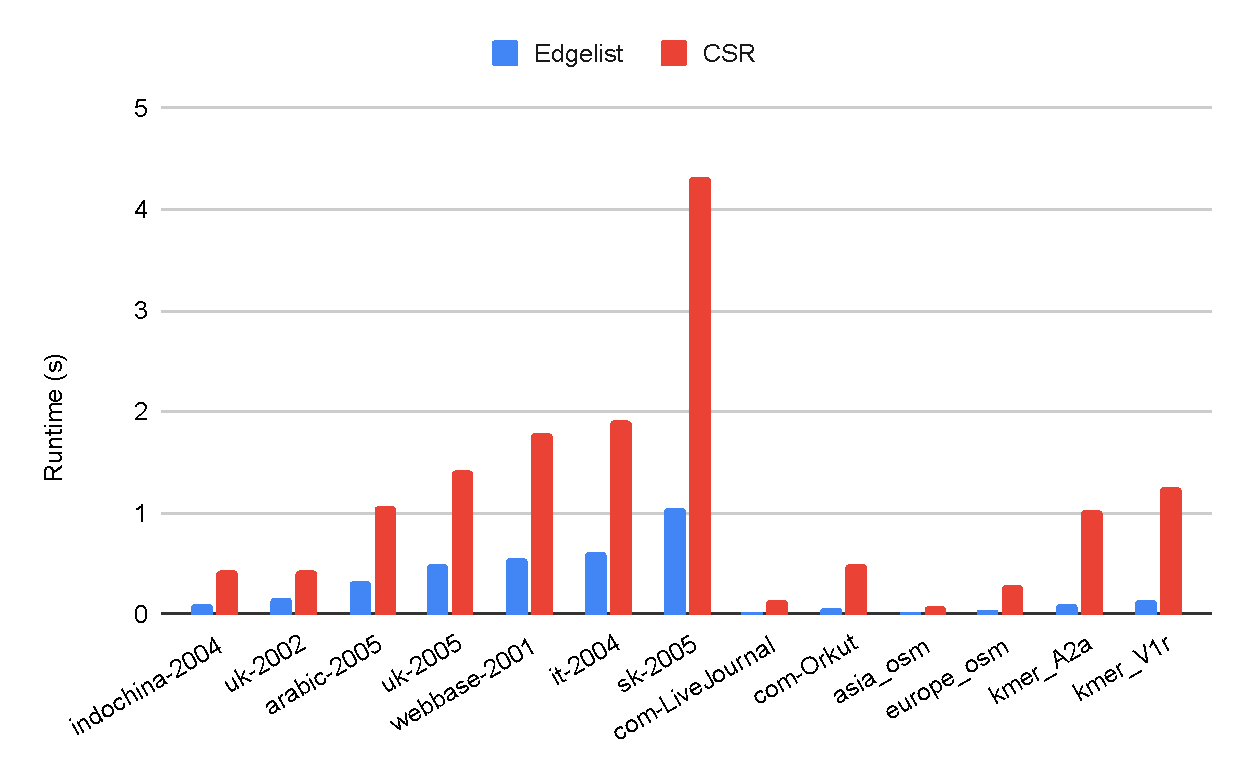
\includegraphics[width=0.68\linewidth]{out/runtime.pdf} \\[-2ex]
  \caption{Time taken by GVEL for edge-list and CSR loading on 13 different graphs.}
  \label{fig:runtime}
\end{figure*}

\begin{figure*}[hbtp]
  \centering
  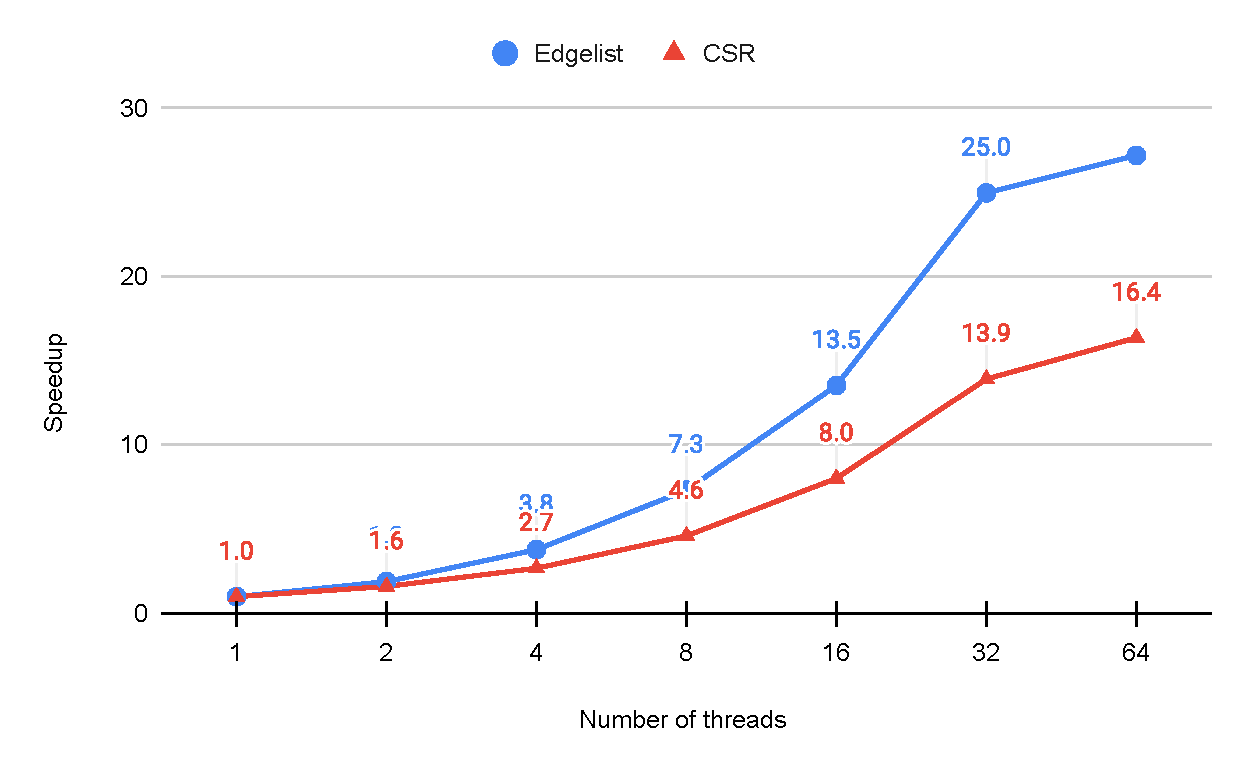
\includegraphics[width=0.68\linewidth]{out/scaling.pdf} \\[-2ex]
  \caption{Speedup of GVEL's Edgelist and CSR loading with increasing number of threads.}
  \label{fig:scaling}
\end{figure*}

\begin{figure*}[hbtp]
  \centering
  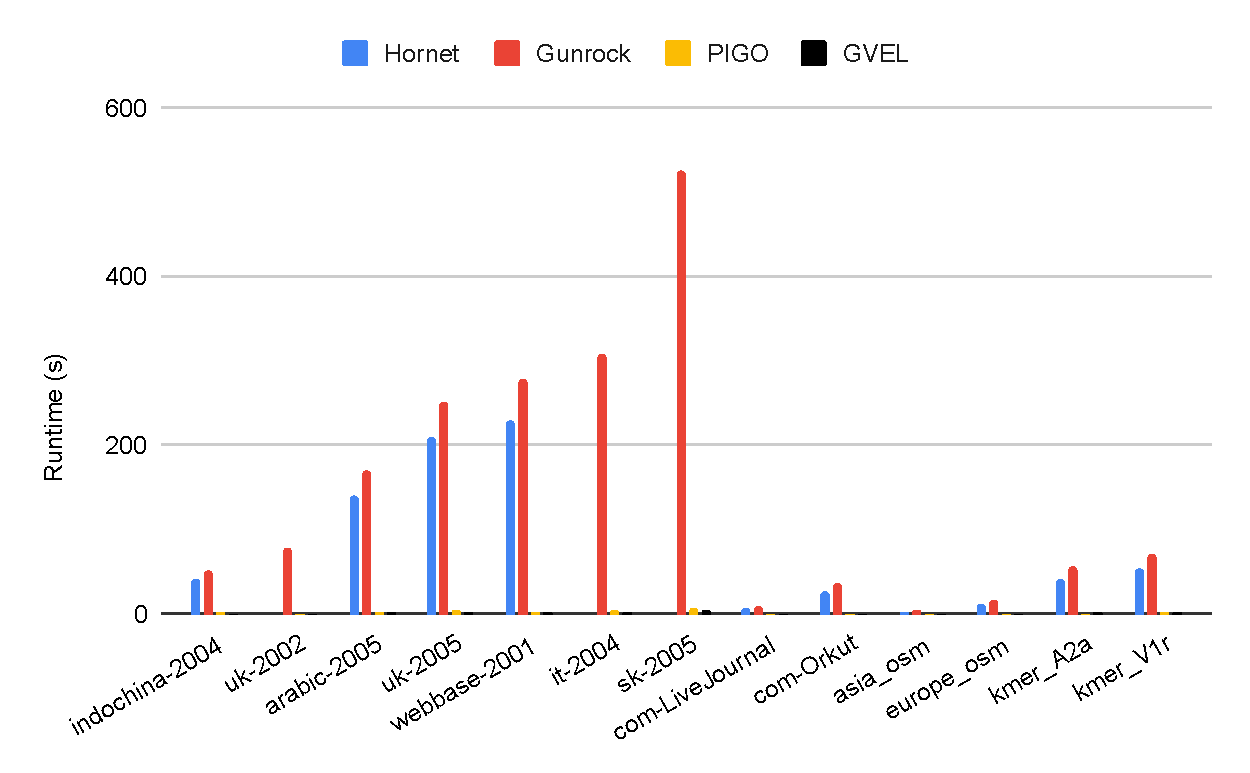
\includegraphics[width=0.68\linewidth]{out/compare-large.pdf} \\[-2ex]
  \caption{Time taken by Hornet, Gunrock, PIGO, and GVEL for reading edge-list and converting it to CSR on 13 different graphs. PIGO and GVEL are not visible on this scale - they are significantly faster than Hornet and Gunrock. The graph loading time for Hornet is not shown for \textit{uk-2002}, \textit{it-2004}, and \textit{sk-2005} graphs as it crashed while loading.}
  \label{fig:compare-large}
\end{figure*}

\begin{figure*}[hbtp]
  \centering
  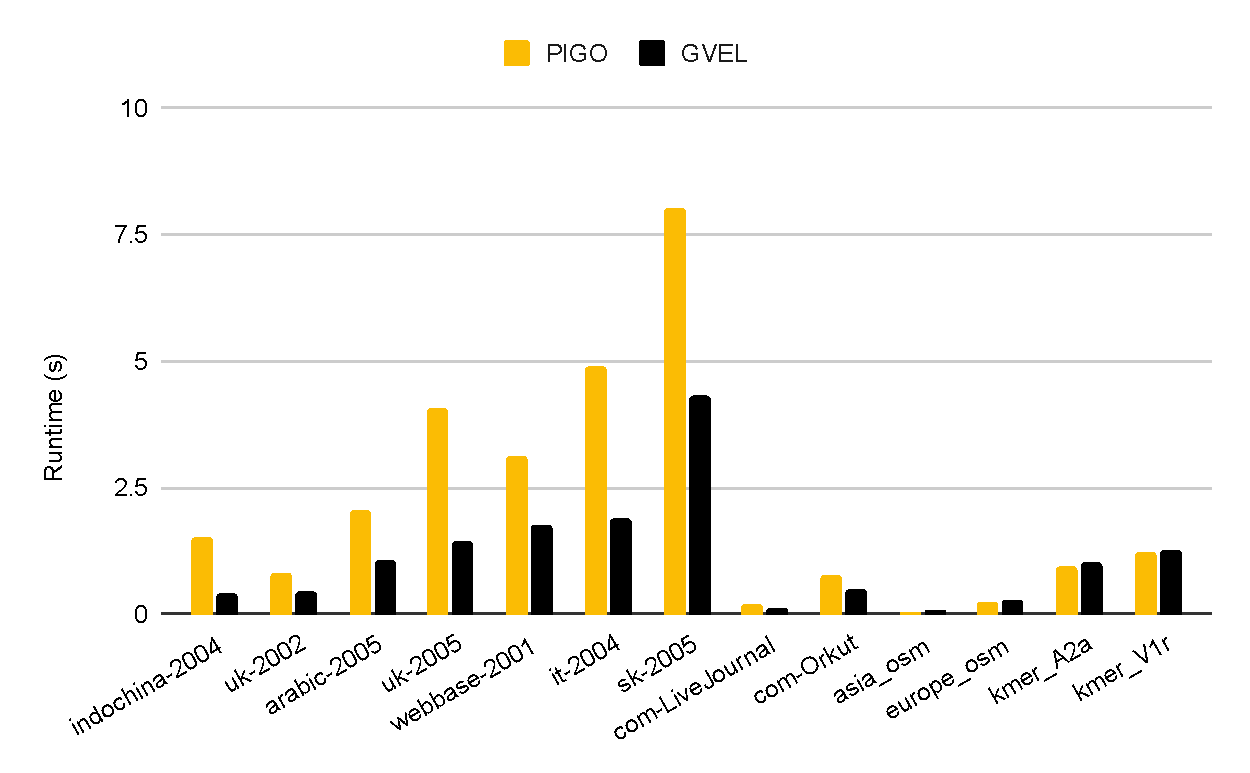
\includegraphics[width=0.68\linewidth]{out/compare-small.pdf} \\[-2ex]
  \caption{Gini coefficient of PageRank values on 24 different graphs, comparing between PageRank values obtained with three different dead-end handling strategies: \textit{teleport from dead-ends} (\textbf{default}), \textit{self-loop dead-ends} (\textbf{loop}), and \textit{self-loop all vertices} (\textbf{loopall}).}
  \label{fig:compare-small}
\end{figure*}



In our comparison with Hornet, Gunrock, and PIGO, we observe that:

PIGO has demonstrated superiority over XXX, prompting our exclusion from the comparison.
The average speedup over Gunrock showcases the efficiency of our approach.
Similarly, the average speedup over PIGO further highlights the performance benefits of our method.
Notably, our approach excels on web graphs characterized by power law distributions and high average degrees.
We present our key findings from the observations in the figure captions.


\textbf{Figure 3}:

The efficiency of reading an edgelist stands out, significantly outpacing the speed of reading a graph stored as CSR, which necessitates an additional conversion step. Surprisingly, the average cost of converting an edgelist to CSR is three times higher than simply reading an edgelist from a file. This underscores the notable speed of modern I/O processes. In the sk-2005 dataset, our approach achieves an impressive reading speed of 1.9 billion edges per second. Notably, it's essential to clarify that the table represents edges as directed, not undirected. To visually represent the edge reading performance across different graphs, we propose the inclusion of a plot illustrating this metric. The sluggishness in CSR reading is justified by its nature as a shared data structure, leading to high contention when multiple threads concurrently attempt to add an edge to the same vertex. The process of adding to CSR structures with small degrees is hampered by false sharing, introducing cache coherency issues that contribute to decreased performance.

We observe that:
- reading edgelist is significantly faster than reading a graph as CSR (this requires and additional conversion step)
- in fact, on average, converting an edgelist to CSR is 3 times more costly than reading and edgelist from file (which is quite surprising indded). This shows that modern IO is fastr (dhooom).
- We are able to read 1.9B edges per second (the table put edges as directed not undirected) in sk-2005.
- Can we have a plot on edge reading performance per graph
- (Justify why CSR reading is slow) converting to CSR is slow becuase it is a shared data structure resulting in high contention beteen thread, when multiple threads attempt to add an edge to the same vertex.
- Also adding to CSR with small degrees suffer from false sharing (cache coherency issue).

\textbf{Figure 4}:



Our observations reveal:

Reading edgelists exhibits impressive scalability, achieving a remarkable 25x scale on 32 threads.
However, at 64 threads, performance is impacted by NUMA effects.
Notably, reading CSR does not scale as well, primarily due to issues such as false sharing and contention.
The influence of NUMA effects is also discernible in CSR reading performance.
The scaling pattern follows multiples of 2 (linear Y-axis, logarithmic X-axis).

% There is a paper called "Efficient Memory Mapped File I/O for In-Memory File Systems" on the topic - where Choi et al. working at Samsung say that mmap() is a good interface for fast IO (in contrast to file streams) and propose async map-ahead based madvise() for low-latency NVM storage devices. The also have a good slides on this - where their (modified) extended madvice obtains ~2.5x better performance than default mmap() by minimizing the number of page faults.
% I tried parsing integers from text and saving into per-thread integer lists. To over-allocate memory for per-thread integer-lists i use sufficient size mmap() instead of malloc(). Even if i over-allocate, due to virtual memory, only memory as much i need is actually used.
